\documentclass[12pt,a4paper]{article}
\usepackage{graphicx}
% \usepackage[english]{babel}
% \usepackage[utf8x]{inputenc}

\usepackage{graphicx} % Required for inserting images.
\usepackage[margin=25mm]{geometry}
\parskip 4.2pt  % Sets spacing between paragraphs.
% \renewcommand{\baselinestretch}{1.5}  % Uncomment for 1.5 spacing between lines.
\parindent 8.4pt  % Sets leading space for paragraphs.
\usepackage[font=sf]{caption} % Changes font of captions.

\usepackage{amsmath}
\usepackage{amsfonts}
\usepackage{amssymb}
\usepackage{siunitx}
\usepackage{verbatim}
\usepackage{hyperref} % Required for inserting clickable links.
\usepackage{natbib} % Required for APA-style citations.


\title{\textbf{ASSIGNMENT 0}}
\author{Sachin Kumar(MC22BT019), Amogh R (CS22BT005)}
\date{}


\begin{document}
\maketitle

\section{Introduction}\label{sec:intro}
In the described scenario, a defending country (DC) aims to secure its border against an attacking country (AC) by deploying a wireless sensor network. The wireless sensors, strategically placed along the border, detect infiltration attempts, enabling the defending country to respond effectively. Key components include the deployment of sensors, real-time communication between them, sophisticated detection algorithms, and a rapid response mechanism involving the deployment of troops. Security measures are essential to prevent tampering, and continuous monitoring and improvement of the sensor network are crucial for its effectiveness. Ethical considerations and adherence to international laws are emphasized in the implementation of defense measures.

\section{Elements of the Scenario}\label{sec:methods}
\subsection{Border}
\begin{itemize}
    \item \textbf{Border Layout:} The border is represented as a long rectangular strip of land, with the length extending to infinity and discretized into a grid.

    \item \textbf{Grid Structure:} The rectangular strip is divided into a grid, with the width consisting of \texttt{W} cells. Each cell in the grid represents a discrete unit of the border.

    \item \textbf{Infinite Length:} While the length of the rectangle is considered infinite, the focus is on the discretized grid structure, which allows for a systematic representation of the border.

    \item \textbf{Geometric Configuration:} The discretization into a grid simplifies the analysis and deployment of a wireless sensor network for border defense, with each cell potentially hosting a sensor for detecting infiltration attempts.
    
\end{itemize}

\subsection{Sensors}
\begin{itemize}
    \item \textbf{Single Sensor per Cell:} Each cell in the border grid is equipped with a motion sensor, capable of detecting moving infiltrators within its own cell.
    
    \item \textbf{Limited Sensing Range:} Sensor detection is confined to its assigned cell; it triggers only if an infiltrator is in motion within that specific cell.
    
    \item \textbf{Energy Conservation:} To extend battery life, sensors employ duty cycling, randomly deciding to be ON or OFF every 10 seconds. This decision is independent and made without communication.
    
    \item \textbf{Random Decision Making:} Sensors make decisions based on a coin flip with a probability $p$ of heads. If heads, the sensor remains ON for the next 10 seconds; otherwise, it turns OFF.
    
    \item \textbf{Independent Operation:} Each sensor operates autonomously, with no communication with other sensors. The initial decision is made at time '0', and subsequent decisions are made independently.
\end{itemize}

\subsection{Infiltrator:}
\begin{itemize}
    \item \textbf{Infiltrator's Movement:} The infiltrator moves in steps, with the ability to choose any of the 8 neighboring cells. Each movement takes 9 seconds.
    
    \item \textbf{Decision and Movement Cycle:} Every 10 seconds, the infiltrator spends 1 second studying neighboring cells and the next 9 seconds moving (if he decides to move).
    
    \item \textbf{Sensor Model Reminder:} The motion sensor model dictates that if the infiltrator decides to move from cell A to cell B, both cells' sensors must be OFF; otherwise, the infiltrator is caught.
    
    \item \textbf{Sensor Status during Movement:} For successful movement, both the departure (cell A) and destination (cell B) sensors must be OFF during the infiltrator's 9-second movement interval.
    
    \item \textbf{Risk of Detection:} If even one of the sensors in cells A or B is ON during the infiltrator's movement, it triggers the motion sensor and leads to the infiltrator being caught.
\end{itemize}


\section{Objective}\label{sec:objective}
The main objective of this problem is to determine the time taken by the infiltrator to cross the border while varying the width of the border and the probability of the sensor being on.

\section{Solution }\label{sec:discussion}
\begin{itemize}
\item We define a \texttt{Clock} class where methods related to time, such as \texttt{getTime()} and \texttt{incrementClockTime()}, are defined to start the clock.


\item Then, we define a \texttt{Sensor} class where a method \texttt{flipACoin()} is defined to handle the sensor's behavior. It mimics tossing a biased coin (with some probability), and turning the sensor on or off based on the bias of the coin.


\item Next, we define a \texttt{Border} class that includes the \texttt{Sensor} within a 2D array.

\item Following that, we define an \texttt{Infiltrator} class where numerous methods are defined. The infiltrator always starts from the point (\texttt{mid},0), where \texttt{mid} is the X-value of the center of the finite border in the simulation. Ideally, this tries to mimic an infinitely long border.

    \begin{itemize}
        \item \texttt{getMotionStatus()}
        \item \texttt{getInfiltrationStatus()}
        \item \texttt{changeMotionStatus(boolean status)}
        \item \texttt{infiltrationSuccess(boolean hasCrossed)}
    
    \item The method \texttt{studySurrounding(Border border)} allows the infiltrator to gather information about the surrounding sensors.
    \item The method \texttt{moveInfiltrator(int pos)} enables the infiltrator to move safely without being caught.
    \end{itemize}
\end{itemize}


\section{Plots}\label{sec:Plot}
\begin{figure}[!htbp]
    \centering
    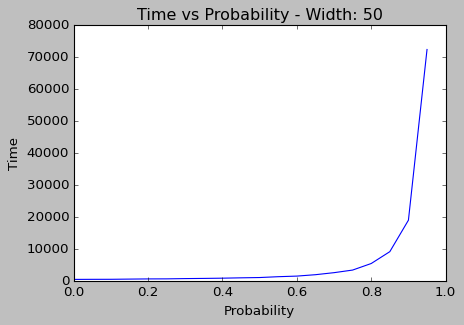
\includegraphics[width=0.5\textwidth]{TvP.png}
    \caption{Average Time taken to cross border vs Probability of sensor turning on}
    \label{fig:example}
\end{figure}
\begin{figure}[!hbpt]
    \centering
    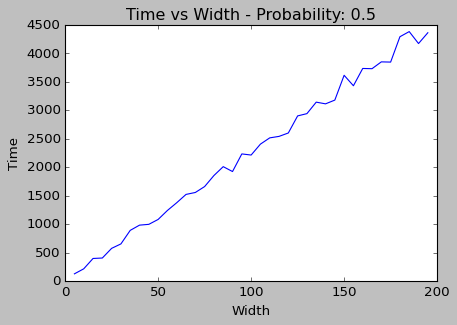
\includegraphics[width=0.5\textwidth]{TvW.png}
    \caption{Average Time taken to cross border vs Width of border}
    \label{fig:example}
\end{figure}
\pagebreak
\begin{figure}[!htbp]
    \centering
    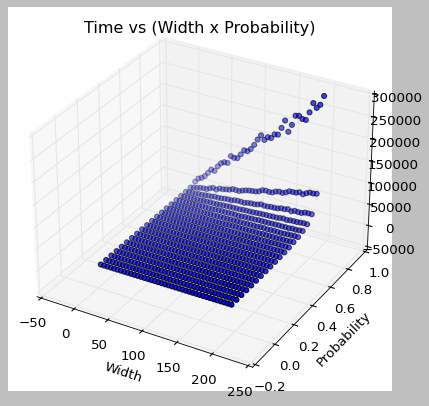
\includegraphics[width=0.5\textwidth]{TvWxP.png}
    \caption{A 3D Plot of Time, Width and Probability}
    \label{fig:example}
\end{figure}

\section{Observation}\label{sec:fObservation}
The following observations can be made from the data collected:
\begin{itemize}
	\item The time taken to cross the border increases drastically as the probability of the sensor turning on reaches the 80\% threshold.
	\item The time taken to cross the border increases linearly with the border width for a fixed probability of the sensor turning on. This is as expected because the average time taken for the infiltrator to make one move does not depend on his position, and rather depends on the probability of the sensors around him turning on/off (kept constant here).
\end{itemize}


\end{document}